% !TEX TS-program = pdflatex
% !TEX encoding = UTF-8 Unicode

% This is a simple template for a LaTeX document using the "article" class.
% See "book", "report", "letter" for other types of document.

\documentclass[11pt]{article} % use larger type; default would be 10pt

\usepackage[utf8]{inputenc} % set input encoding (not needed with XeLaTeX)
\usepackage{graphicx}
\graphicspath{ {images/} }
%%% Examples of Article customizations
% These packages are optional, depending whether you want the features they provide.
% See the LaTeX Companion or other references for full information.

%%% PAGE DIMENSIONS
\usepackage{geometry} % to change the page dimensions
\geometry{a4paper} % or letterpaper (US) or a5paper or....
% \geometry{margin=2in} % for example, change the margins to 2 inches all round
% \geometry{landscape} % set up the page for landscape
%   read geometry.pdf for detailed page layout information

\usepackage{graphicx} % support the \includegraphics command and options

% \usepackage[parfill]{parskip} % Activate to begin paragraphs with an empty line rather than an indent

%%% PACKAGES
\usepackage{booktabs} % for much better looking tables
\usepackage{array} % for better arrays (eg matrices) in maths
\usepackage{paralist} % very flexible & customisable lists (eg. enumerate/itemize, etc.)
\usepackage{verbatim} % adds environment for commenting out blocks of text & for better verbatim
\usepackage{subfig} % make it possible to include more than one captioned figure/table in a single float
% These packages are all incorporated in the memoir class to one degree or another...

%%% HEADERS & FOOTERS
\usepackage{fancyhdr} % This should be set AFTER setting up the page geometry
\pagestyle{fancy} % options: empty , plain , fancy
\renewcommand{\headrulewidth}{0pt} % customise the layout...
\lhead{}\chead{}\rhead{}
\lfoot{}\cfoot{\thepage}\rfoot{}

%%% SECTION TITLE APPEARANCE
\usepackage{sectsty}
\allsectionsfont{\sffamily\mdseries\upshape} % (See the fntguide.pdf for font help)
% (This matches ConTeXt defaults)

%%% ToC (table of contents) APPEARANCE
\usepackage[nottoc,notlof,notlot]{tocbibind} % Put the bibliography in the ToC
\usepackage[titles,subfigure]{tocloft} % Alter the style of the Table of Contents
\renewcommand{\cftsecfont}{\rmfamily\mdseries\upshape}
\renewcommand{\cftsecpagefont}{\rmfamily\mdseries\upshape} % No bold!

%%% END Article customizations

%%% The "real" document content comes below...

\title{Face Tracking for Optimized Bitrate Control in Low Delay Video Encoding}
\author{Chethan Ningaraju}
%\date{} % Activate to display a given date or no date (if empty),
         % otherwise the current date is printed 

\begin{document}
\maketitle
\clearpage
\tableofcontents
\clearpage
%%%
%%%%INTRODUCTION
%%%%
\section{Introduction}
	In recent years, there is increasing demand for high quality video conferencing solutions. To address this growing need there has been constant improvement in  low delay video coding techniques along with better techniques to ensure low delay transmission reliability at the network level. The tremendous increase in smart phone usage has led to increase in video telephony over cellular networks whose bandwidth is highly constrained. Therefore, it is very important to develop methods of delivering high quality video with less bandwidth requirement. This work explores the methods of region of interest(ROI) based encoding to exploit the available bandwidth to encode regions that are of high importance to perceptual quality with higher quality. 

The goal of this work is to identify the salient region of a frame, which is the face of the participant in a video conference. In a first iteration we assume ideal capture conditions so that the results of the face tracking will be directly used as side information for the H264/AVC encoder's bitrate-control. Face regions should allocate an above-average bitcount and yield a better visual quality than background regions. It is also the aim of this work to develop and extensively evaluate the strategy of uneven bitrate allocation and also to identify its limitations.
  \subsection{Low Delay Bitrate Control}
	The bitrate control module is responsible for controlling the bit-consumption of the encoder to guarantee smooth playback. Bitrate control module is not codec specific and operates independent of any chosen codec. Figure \ref{fig:Bitrate Control Module Functionality} shows the functionality the bitrate control module. The main purpose of the bitrate control module is to ensure smooth playback of the encoded video under given bandwidth and delay constraints.  It achieves this by controlling the quantization parameter (QP) used during the encoding. The decision of quantization parameter is done considering the input bitrate, framerate, input complexity (spatial and temporal activity) and acceptable input delay. The module also takes the feedback from the encoder regularly to make better QP decision.  The feedback from the encoder gives information about the content of the video and helps the module to decide the right QP for a given bit budget.
\begin{figure}[h]
    \centering
    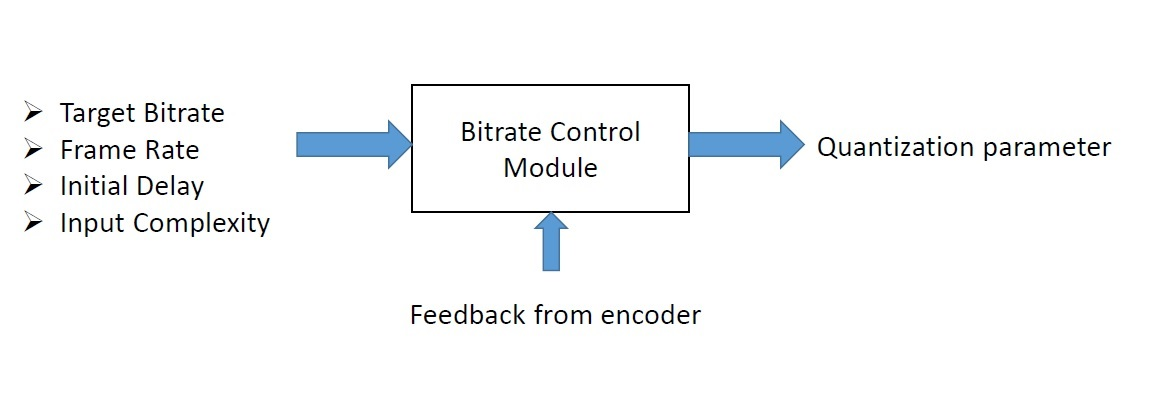
\includegraphics[scale=0.5]{RC_block}
    \caption{Bitrate Control Module Functionality}
    \label{fig:Bitrate Control Module Functionality}
\end{figure} 

The need for extremely low end to end delay in video telephony puts additional constraints on video coding which results in compromise of video quality. During the low delay video encoding, tools like bi-directional prediction are disabled. The delay in video encoding is a direct measure of Video Buffer Verifier (VBV) buffer size of rate control. The VBV buffer is a virtual buffer modelled by the bitrate control module to ensure that video stream can be correctly buffered, and played back at the decoder end. This can be visualized as a leaky bucket, where the output of encoder with variable rate is stored in a leaky bucket which is draining at a constant rate. Any underflow or over flow in this buffer must be avoided to ensure smooth playback. When the size of the VBV buffer is very low (due to low delay), there is less room to accommodate the variation in bitrate of the encoder. This implies that there can be minimum variation in the size of frame irrespective of the content. To ensure this, encoder's quantization parameter (QP) is adapted on a macroblock level in order to ensure that the maximum allowed bitcount for an encoded frame is not exceeded.

The bitrate control algorithm computes the QP for a given macroblock based on two factors. 
\begin{itemize}  
\item Activity of the macroblock - Difference of actual and predicted macroblocks.
\item Current Virtual Buffer occupancy.
\end{itemize}

%%SubSub section for detailed overview of bitrate control	
\subsubsection{Overview of Bitrate Control Module}
	The bitrate control module used in this work in a modified version of \cite{JVTF086}. As mentioned earlier quantization parameter at a macroblock depends on 2 factors. First, a delta QP (dqp) is calculated considering the

  \subsection{ROI based coding}
	In conventional video coding, all regions of a frame are considered equally important. It is assumed that all the regions contribute equally to the perceptual quality. Some video codecs use the fact that high frequency components are less important to the human visual system and perform preferential coding based on spatial frequency. The higher frequency components which are not so important to perceptual quality is encoded with higher QP. However, such preferential coding does not take into account the contents of the frame to be encoded. 

The study of Human Visual System (HVS) also shows that human eyes can only focus at one area in a frame at any given point in time which is called region of interest. Region of interest based coding is not a common practice in video coding because it is very hard to automatically detect important regions that contribute the most to the perceptual quality. This is because the region of interest constantly keeps changing depending on the content. For instance, in a movie, the region of interest can depend on context of the scene. Developing generic techniques for detection of ROI in such videos is very difficult. However, region of interest in the video conferencing content is going to be the face region predominantly. Due to recent improvements in face detection algorithms it is possible to detect the face with good accuracy. The study in \cite{HighQualityROICodingForVideoConferencing} shows how boosting quality of face regions can improve the overall perceived quality of the video. This work aims to study possible ways of improving perceptual quality of the video by detecting face regions and coding it with higher quality than rest of the frame.

 As mentioned earlier, the bitrate control allocates bits at every macroblock and adjusts the QP. In a simple approach one would try to distribute the bitrate evenly on every macroblock. Since load efficiency is of high importance it is not advisable to do multipass encoding for optimal bitrate allocation. Therefore, over-allocation in one macroblock has to be compensated by under-allocation (using a higher QP) for neighboring macroblocks, regardless of the image content. However, a more intelligent allocation strategy should take the image content into account. Thus parts of the image with higher importance (e.g.faces) should be given a higher percentage of the overall bitcount which results in higher visual quality. Background regions would get a lower proportion of the bitcount.

\section{Study setup}
\subsection{codec configuration}      
This work uses Citrix h264 video codec for the study. The encoder is configured in low delay mode suitable for video conferencing and other real-time applications. The encoder is configured to use IPPP mode with intra/key frames encoded only at the beginning of the sequence followed by uni-directional P frames. Due to low delay there is no provision to re-encode the frame in case of buffer overflow. The frames are skipped/dropped entirely in case of buffer overflow to guarantee smoother playback by maintaining the delay constant. 
\subsection{Measurements}
One of the crucial aspects in this study is the metric used to evaluate various algorithms in order to choose the best approach. The goal of this study is to improve the quality of the ROI region at the cost of degrading the non-ROI regions. Since the whole approach is to measure the gain in perceptual quality, using frame level PSNR alone as a metric could be misleading. 

In this study, the difference in average PSNR of frames and average ROI PSNR is used as one of the metrics to evaluate different algorithms. The expectation is to see an improvement in ROI PSNR, with degradation in PSNR of the non-ROI regions. The shift in the quality of ROI and non-ROI regions should be achieved keeping the bitrate unchanged. Therefore, the second aspect is to measure the deviation in bitrate behavior from the original output. Third aspect involves the measurement of PSNR and QP distribution within a frame. This is to ensure structure of the face is recognizable in the QP map which implies face region information is used to alter the behavior of QP allocation. The PSNR quality map is required to ensure that there is visible difference in quality of ROI without badly degrading the quality of non-ROI. 

To measure all these behaviors following metrics are considered
\begin{itemize}  
\item Quality metrics - PSNR of ROI and non-ROI regions.
\item PSNR and QP variation within the frame.
\item Delay plot comparison for the entire sequence.
\end{itemize}
\subsubsection{Quality metrics}
The initial approach is to find the gain in PSNR of ROI, however finding the desirable extent of improvement in PSNR of ROI along with acceptable drop in PSNR of non-ROI is tricky. The idea here is to find the right balance between quality improvements in ROI with degradation of non-ROI region as to achieve maximum perceptual quality. The values in Table \ref{InitPSNR1} shows the PSNR values of original output before any modification with respect to ROI based encoding was done. It is clear that the overall PSNR of ROI is much lower compared to that of the overall frame PSNR. This is not a desirable state to be in since the regions that matter most to perceptual quality have lesser PSNR on average.

%Original results
\begin{table} [h!]
\centering
\begin{tabular}{ |c|c|c| }
 \hline
Content & PSNR Avg (dB) & PSNR ROI (dB) \\
 \hline 
 Paul640x480, 250kbps & 39.22 & 37.54 \\ 
 Johny1280x720 750kbps & 40.90 & 39.20 \\  
 \hline
\end{tabular}
 \caption{Initial PSNR values}
 \label{InitPSNR1}
\end{table}

The PSNR is calculated using weighted sum of PSNR of individual components per picture (PSNR\textsubscript{Y}, PSNR\textsubscript{U} and PSNR\textsubscript{V}) \cite{ComparingCodingEfficiency}.
\begin{equation}
\label{Eq:PSNR}
PSNR\textsubscript{YUV} = ( 6 . PSNR\textsubscript{Y} + PSNR\textsubscript{U} + PSNR\textsubscript{V}) / 8
\end{equation}
 where individual components are computes as
\begin{equation}
\label{Eq:PSNRDef}
PSNR = 10 . log_{10}((2^B - 1)^2 / MSE)
\end{equation}

where, B = 8 is the number of bits per sample of the video and MSE is the mean squared error.

 The change in PSNR of ROI region and non- ROI region is measured as average of PSNR of entire frame and average of PSNR of ROI region of all the frames in the sequence. This measure will also indicate the aggressiveness of an algorithm. The study also included average MSE based PSNR which is calculated by accumulating the MSE over entire sequence and then calculating the PSNR, this metric was found to be heavily influenced by the outliers and hence not presented in the results in this study.
\subsubsection{PSNR and QP Variation}
The study of PSNR and QP distribution within the frame is important to understand the effect of bit movement from ROI to non-ROI regions. The PSNR and QP is extracted at the macroblock level. It is then stored in the raster scan order which can be used to display as  an image to compare the structure with that of the video frame. These values are represented as a gray scale image with values between 0 to 255. 

\begin{figure}[!h]
    \centering
%Raw YUV image
    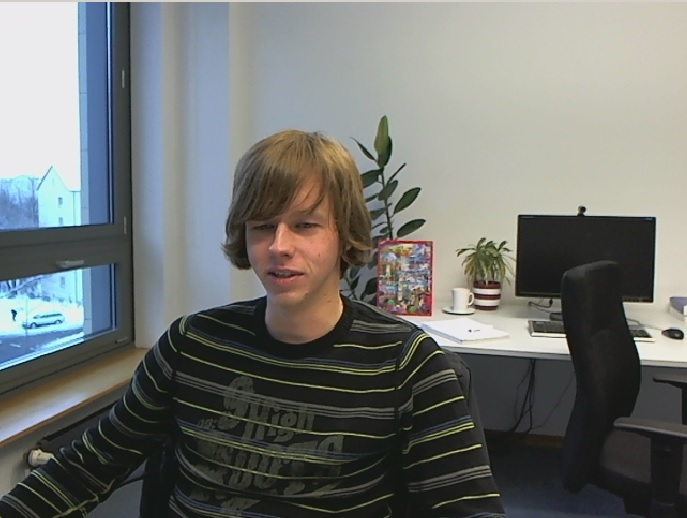
\includegraphics[scale=0.5]{PaulDefault120}
    \caption{A Frame in the sample video}
    \label{fig:PaulDefault120}
%%encoded frame image
    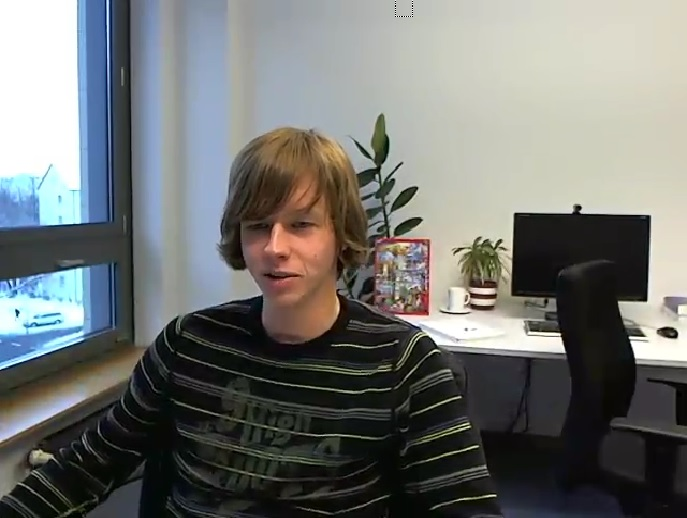
\includegraphics[scale=0.5]{PaulDefault120_91250kbps}
    \caption{Sample frame in encoded video (250kbps)}
    \label{fig:PaulDefaultencoded}
\end{figure} 

In a QP scale map, the darker regions in a frame indicate higher quantization. Even though quantization parameter used for a block to be encoded is closely related to the PSNR of the block, it is not the only deciding factor. The PSNR can also vary depending on the content. Generally, the lower frequency regions have better PSNR even when encoded with a higher QP. Also when a region of the frame is static, it tends to have better PSNR even when higher QP is used because of very less new information to be encoded. Therefore, the PSNR distribution within a frame represented as a gray scale image is also included to analyze the effect of bit movement within the frame.

The image in figure \ref{fig:PaulDefault120} shows a frame in the sample video conferencing content with resolution of 640x480 and 30 frames per second. The image in figure \ref{fig:PaulDefaultencoded} shows the same frame when encoded with the codec configurations discussed in previous section with 250 kbps bitrate. The reason for considering a low bitrate of 250 kbps is that it will help in making the improvement in face region and decrease in quality of background more evident and hence will be useful in evaluating different algorithms. 

\begin{figure}[!h]
    \centering
    
\includegraphics[scale=0.5]{PaulDefault120_91250kbps_quant}
    \caption{Quantization map}
    \label{fig:PaulDefault120Quant}
    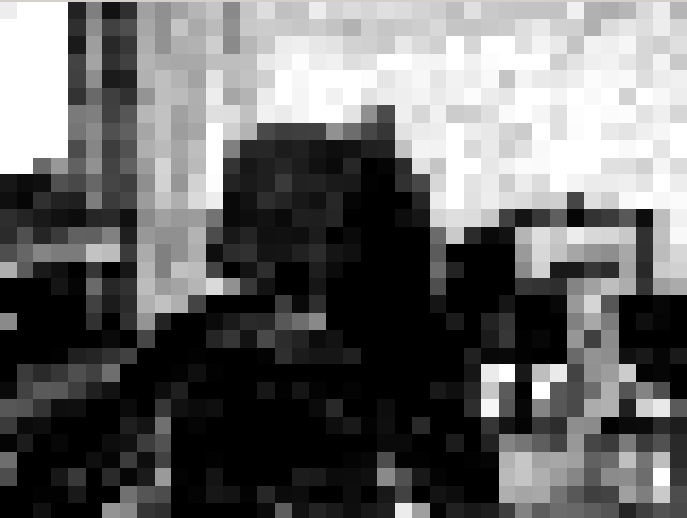
\includegraphics[scale=0.5]{PaulDefault120_91250kbps_psnr}
    \caption{Relative PSNR map}
    \label{fig:PaulDefault120PSNR}
\end{figure} 

The image in figure \ref{fig:PaulDefault120Quant} shows the quant map of the frame in figure \ref{fig:PaulDefaultencoded}. The darker regions in this map indicate usage of higher quantization parameter compared to the lighter regions. It can be noticed that since no information about region of interest is used while encoding the frame, the pattern of quantization appears almost random. The shape of the original content is almost not recognizable from the quantization map.

The image in figure \ref{fig:PaulDefault120PSNR} shows the PSNR for the frame in figure \ref{fig:PaulDefaultencoded}. This map is identical to the quantization map, the lighter regions here represent the regions with higher PSNR, the darker regions indicate lower PSNR and worser quality. This map is relative within the frame and does not represent  absolute quality. This map is generated by considering the full range of PSNR of the image after removal of outliers. The map is generated by mapping the PSNR range between 10th percentile and 90th percentile of the whole frame to value between 0 to 255. Such PSNR maps with absolute scale is also studies to compare results across different configurations. 

It is evident that the structure of the original content is preserved in the PSNR map. The background regions have better PSNR, the foreground has worser quality and the difference in quality is quite huge. The difference in the quality is due to the fact that, background in a video conferencing content is mostly static and hence gets encoded better with every frame. On the other hand, the foreground has motion and new data to be encoded, and hence it cannot achieve the same quality as background. Since the focus of attention during video telephony is foreground or the face region, improving the face region must help in improving overall perceptual quality. The effect of such preferential encoding is studied in this work. The idea is to reduce the PSNR difference between foreground and background and to boost the quality of face to same level as background if not better.
%%
%%Bitrate Fluctuation and delay plots
%%
\subsubsection{Bitrate fluctuation - Delay plots}
The core idea of this study is to efficiently use the bits within the frame to encode region of interest. The algorithms used to achieve that purpose should not alter the overall behavior of the codec in terms of bit consumption. As mentioned in previous sections, the codec skips the frame in order to maintain strict VBV buffer compliance. Skip frames result in jerky playback and hence should be avoided as much as possible. The intelligent bit-allocation scheme should not contribute to more skip frames if not reduce them.

A plot of measuring the delay of each frame is used to verify this. Figure \ref{fig:PaulDefault250kbpsDelay} is the delay plot of bitstream encoded with 250 kbps (a sample frame in figure \ref{fig:PaulDefaultencoded}). Every point in the plot specifies the time taken by the corresponding frame of x-axis to reach the decoder assuming zero transmission delay. The curve appears mostly smooth except for sudden drops (zero values). These zero value points indicate skip frames. Since these frames are not included in the final bitstream and hence not transmitted, the delay is indicated as zero. 
\begin{figure}[!h]
    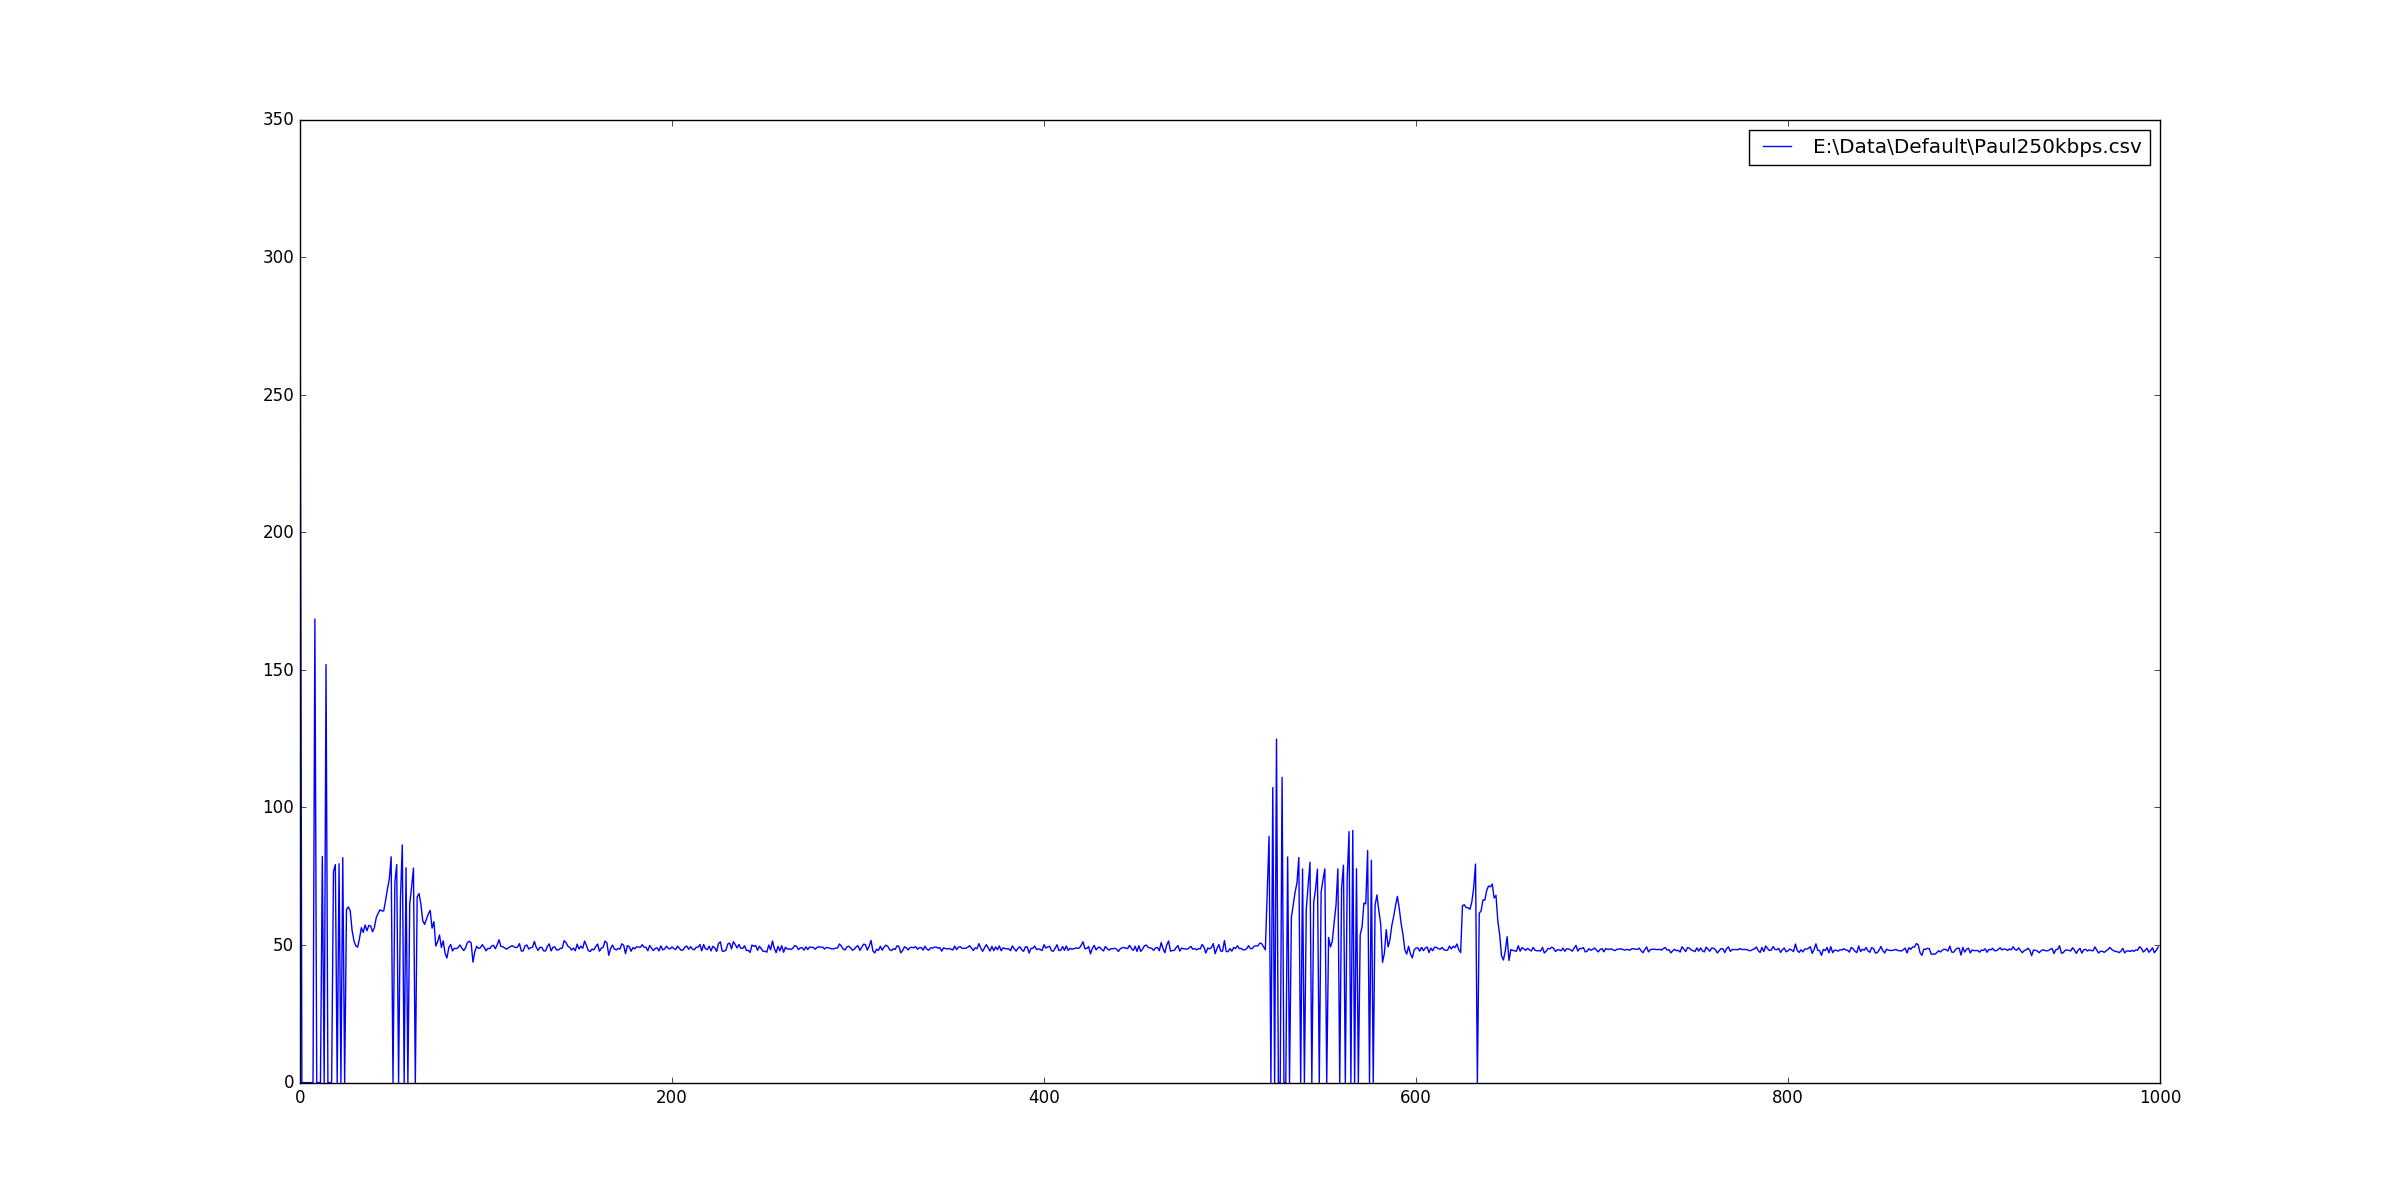
\includegraphics[scale=0.25]{PaulDefault250kbpsDelay}
    \caption{Delay plot}
    \label{fig:PaulDefault250kbpsDelay}
\end{figure} 
Ideally, an algorithm with intelligent bit allocation within a frame should not alter the shape of this graph. It is also desirable to not have any increase in the number of skip frames. Since, the algorithm is not expected to change overall behavior it is not expected to have reduction in number of skip frames.
%
%Face Detection
%
\section{Face Detection}

Face detection algorithms are used to mark the region of interest in the current frame. All the algorithms considered for intelligent bit allocation involve improving the region of interest at the cost of rest of the frame. Therefore, it is very important to have high reliability with face detection. Any false detection will lead to degradation of the actual region of interest compared to normal encoding, this should be avoided in all scenarios. The damage caused by false detection is higher than the loss due to not detecting any face. Therefore, a high threshold must be used to declare any region of the frame as face.
\begin{figure}[!h]
    \centering
    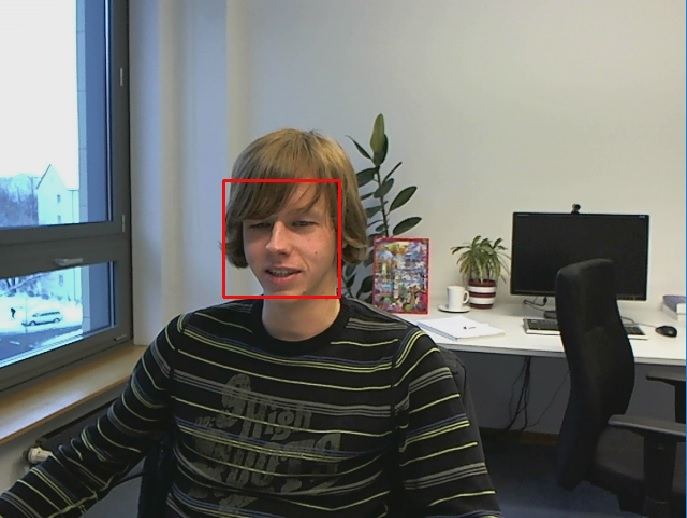
\includegraphics[scale=0.4]{PaulDefault120FaceRecognized}
    
\includegraphics[scale=0.4]{PaulDefault120FaceMap}
    \caption{Face Detection binary map}
    \label{fig:PaulDefault120FaceMap}
\end{figure}

 The face detection module itself shall not be a part of the encoder, but the output from the face detection is a binary file with face regions marked is used as input by the encoder. In this work, the face detection module uses input YUV to the encoder and marks the region of interest at the macro block level. Each byte value in the output file of face detection module represents a macro-block scanned in raster scan order. A value of 0xff signifies macro-block being part of the face or region of interest and 0x00 represents a normal macro-block. Figure \ref{fig:PaulDefault120FaceMap} represents the face map generated for the frame shown in Figure \ref{fig:PaulDefault120}. The region in white is considered as region of interest, this information is used inside the bitrate control module of the encoder to perform intelligent bit allocation.

Different approaches are used to detect the face region in the video. There is always a trade-off between accuracy of face detection algorithm and its complexity. The work presented here is mostly relevant to real time systems. Any added complexity due to additional module of face detection will cause significant delay which is totally unacceptable in such systems. Therefore, the algorithm chosen for face detection must be light weight and reasonably accurate in all lighting conditions. 

\subsection{Spatial Domain Face Detection}
In this approach, the face detection algorithms work directly on the pixel values. This approach is simple in terms of implementation. Many open-source solutions like OpenCV offers a ready to use solution that can be integrated with the codec library. It has large set of trained classifiers considering many types of faces and viewing angles. However, this is a computation intensive approach and almost impractical to use in the final solution. 
\subsection{Compressed domain Face Detection}
Most available face detection algorithms work on the pixel domain. These algorithms provide good level of detection accuracy. The main drawback of this approach is that they are computationally intensive. As discussed earlier, the use case considered in this work has very less room for additional computations. Therefore, in this work ways of compressed domain face detection is explored to detect faces with less computational requirements. 
Many works have been published
TBD LATER
%
%Different approaches
%
% 
\section{ROI based Intelligent Bitrate Control - Approaches}
There are many ways of using the additional information of knowing the region of interest. These methods should increase the quality of the ROI to gain maximum perceptual quality.
\subsection{QP offset}
The simplest and straight-forward way of creating a bias in quality for ROI and non-ROI is by using a QP offset between macroblocks belonging to these regions in the existing bitrate control module. The feedback from the encoder to rate control module will ensure that final bitrate is still met. A negative QP offset  is used for ROI regions, which triggers increase in QP of non-ROI regions due to the feedback. 

Such QP offsets will ensure the quality difference and shall not be overruled by bitrate control mechanisms. However, this approach might result in bitrate control over-reacting for the blocks around the ROI and encode them with extremely low quality. The magnitude of QP offset shall dictate the magnitude of shift in quality for the ROI. This approach is used to find right QP offset for best perceptual quality. 

It is perhaps a better idea to link the confidence quotient of face detection algorithms with the QP offset used. It should also be dependent on the area of the face, if the area of the ROI is considerably large in a video then the quality difference should be minimized. This is because there will be lesser non-ROI regions to compensate for additional bits used in ROI.
\begin{figure}[!h]
    \centering
    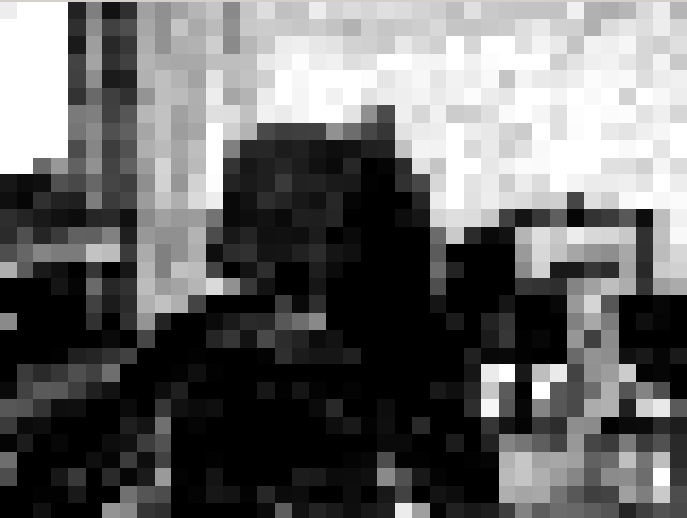
\includegraphics[scale=0.4]{PaulDefault120_91250kbps_psnr}
    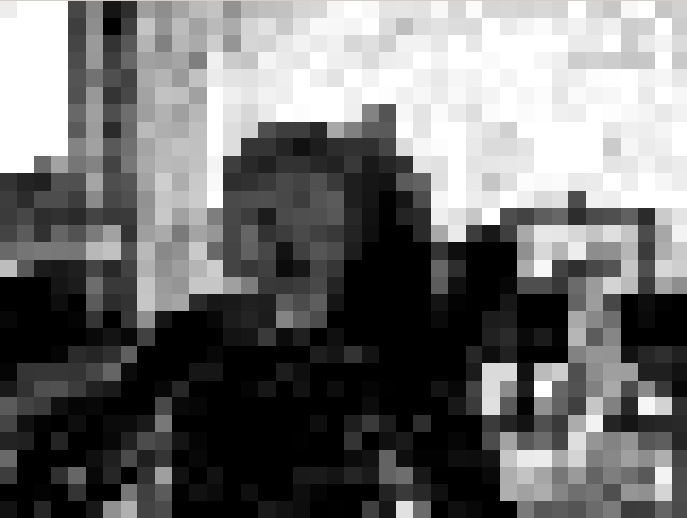
\includegraphics[scale=0.4]{QPOffset/paul120_250kbps_QPoffset4_psnr}
    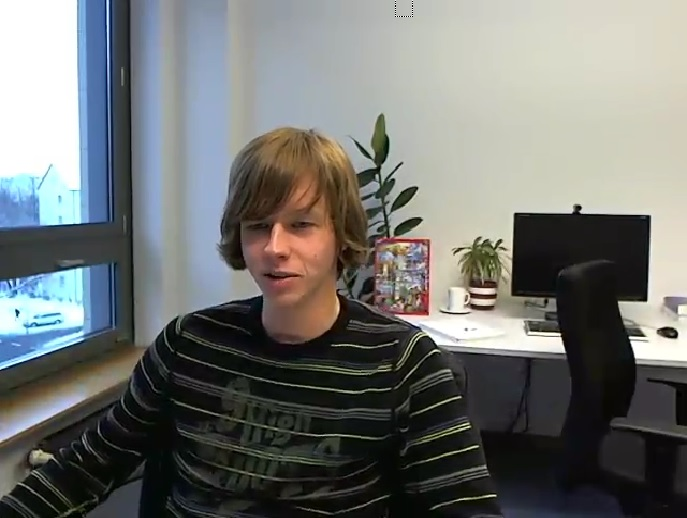
\includegraphics[scale=0.4]{PaulDefault120_91250kbps}
    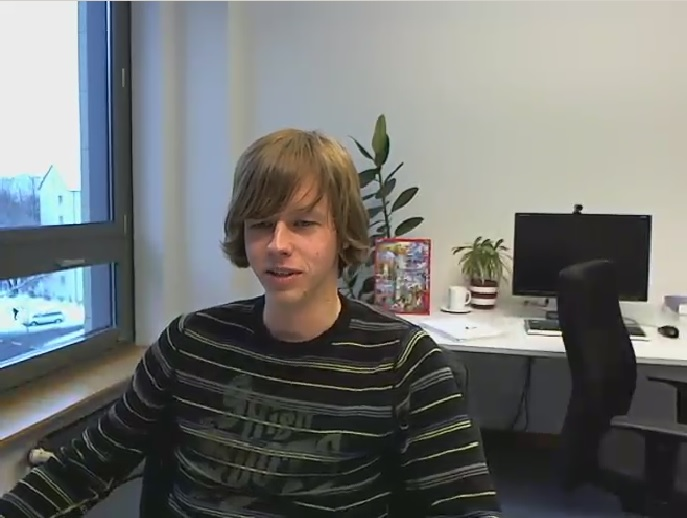
\includegraphics[scale=0.4]{QPOffset/paul120_250kbps_QPoffset4}
    
\includegraphics[scale=0.37]{PaulDefault120_91250kbps_quant}
    
\includegraphics[scale=0.4]{QPOffset/paul120_250kbps_QPoffset4_quant}    
    \caption{Comparing the images with QP offset of 4 for ROI}
    \label{fig:Default_QPOffsetCompare}
\end{figure}

\begin{figure}[!h]
    \centering
    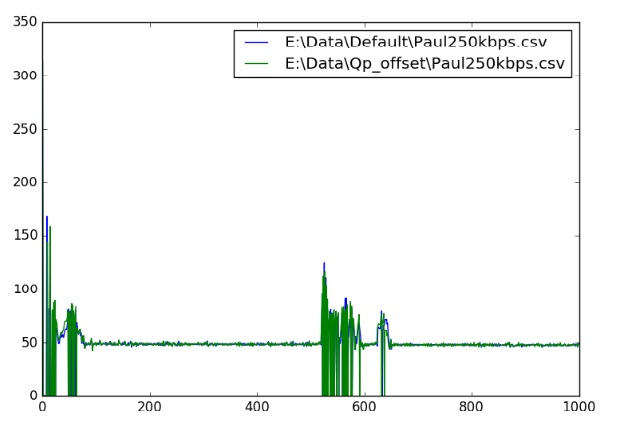
\includegraphics[scale=0.75]{QPOffset/Paul250kbps_QP_Offset_Delay}
    \caption{Delay Comparison of images with QP offset of 4 for ROI}
    \label{fig:DelayDefault_QPOffsetCompare}
\end{figure}

The images in \ref{fig:Default_QPOffsetCompare} shows the comparison between sample frame from original video with video encoded using QP offset of -4 for the ROI region and their corresponding attributes like PSNR map, Quant map. It can be seen that the QP in ROI region is considerably low compared to non ROI regions (marked with lighter shade of gray). The PSNR of the face is now more closer to the background region. The face appears much sharper due to additional boost in quality. The overall bitrate of the streams remained almost the same, the difference in the result is only due to the movement of bits. The number of dropped or skip frames were found to be same as original video. Figure \ref{fig:DelayDefault_QPOffsetCompare} shows the comparison of delay of original bitstream with the bitstream with QP offset for ROI. It can be seen that the delay behavior does not change significantly with skip/dropped frames at same locations.

The results of ROI based PSNR is tabulated in Table \ref{AllPSNR1}. It can be noticed that the ROI PSNR now approaches the overall frame PSNR. This difference can be further altered by tuning the QP offset used.
\begin{table} [h!]
\centering
\begin{tabular}{ |c|c|c|c| }
 \hline
Methodology & Content & PSNR Avg (dB) & PSNR ROI (dB) \\
 \hline 
QP Offset & Paul640x480, 250kbps & 38.90 & 38.88 \\ 
 & Johny1280x720 750kbps & 40.49 & 40.22 \\  
 \hline
Reaction Factor & Paul640x480, 250kbps & 38.22 & 39.50 \\ 
 & Johny1280x720 750kbps & 39.71 & 40.74 \\  
 \hline
\end{tabular}
 \caption{PSNR Comparison for different approaches}
 \label{AllPSNR1}
\end{table}

%
\subsubsection{Tuning QP Offset}
As mentioned earlier, the methods discussed in this work only aim to re-distribute the bits within a frame based on region of interest. The extent of re-distribution should be carefully chosen to avoid degradation of the background to an extent that artifacts become noticeable to the viewer even though they are not expected to concentrate on those regions. Ideal level of redistribution will make sure that there is maximum transfer of bits from non-ROI region to ROI without creating any visible artifacts in the image.
\begin{figure}[!h]
    \centering
    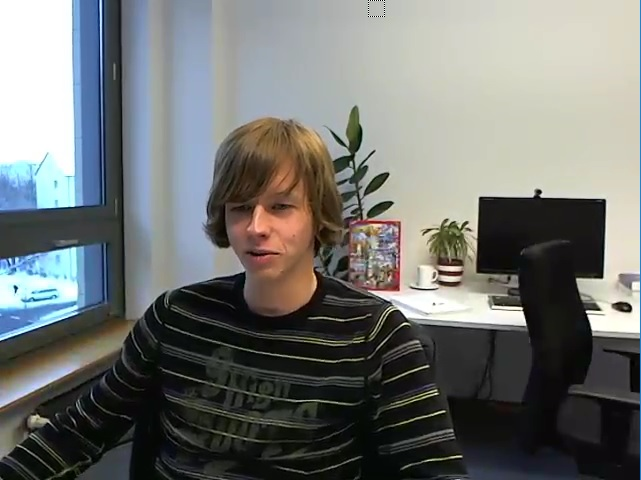
\includegraphics[scale=0.43]{QPOffset/trialOffset/Paul250kbps_offset2}
    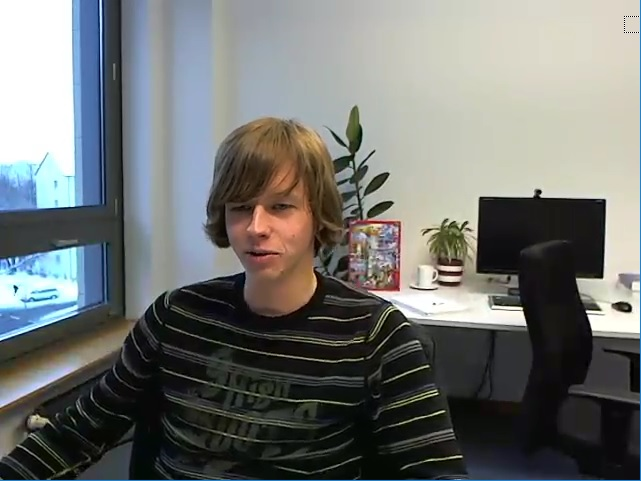
\includegraphics[scale=0.43]{QPOffset/trialOffset/Paul250kbps_offset4}
    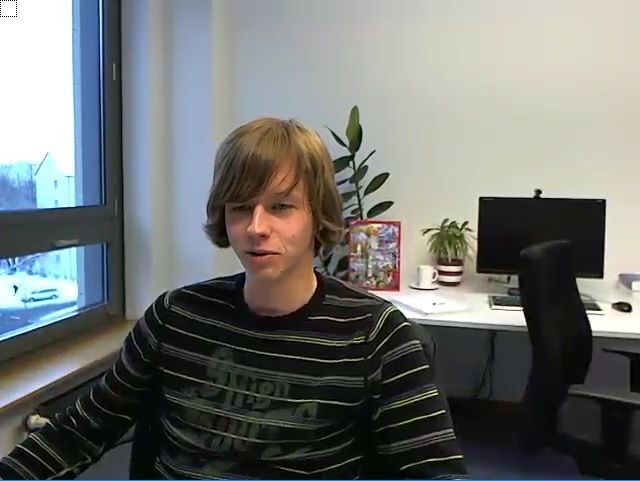
\includegraphics[scale=0.43]{QPOffset/trialOffset/Paul250kbps_offset6}
    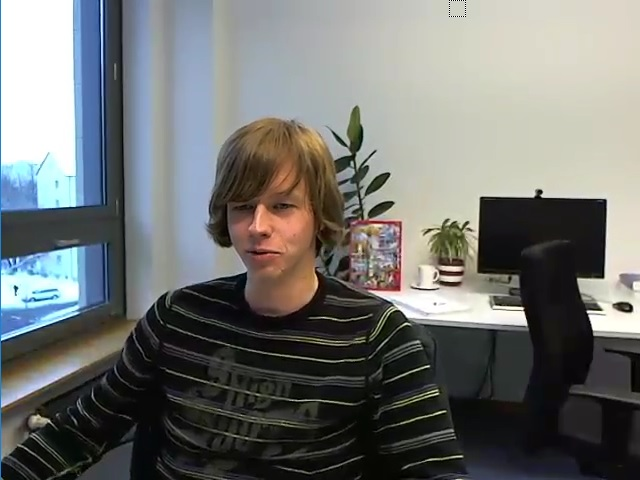
\includegraphics[scale=0.43]{QPOffset/trialOffset/Paul250kbps_offset8}  
    \caption{Tuning QP offset - Trial QP offsets used are 2, 4, 6 and 8 in raster scan order}
    \label{fig:Default_QPOffsetTuning}
\end{figure}
\begin{figure}[!h]
    \centering
    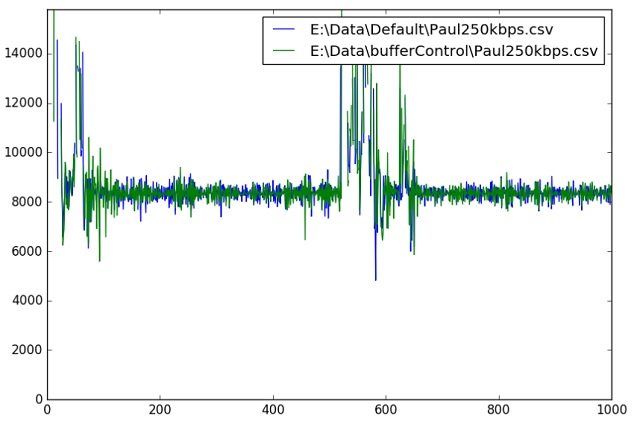
\includegraphics[scale=0.75]{BufferControl/Paul250kbps_Buffer_Control_Delay}
    \caption{Delay Comparison of original video with ROI based reaction factor modification}
    \label{fig:DelayDefault_BufferControltCompare}
\end{figure}

In this work, various offsets were used to study the effect of magnitude of QP offset on perceptual quality. The results shown in Figure \ref{fig:Default_QPOffsetTuning} shows that, as QP offset increases the face region appears more sharper which improves the overall perceptual quality of the frame. The image with QP offset of 8 appears to not have any noticeable blockiness in the background. However, using a very high QP offset triggers another problems that is not shown in the sample images. Due to increased QP offset, the encoder is forced to use lower QP even when virtual buffer is critically full. This increases the number of skipped/dropped frames in the entires sequence. The sample video consisted of 1000 frames and a total of 44, 46, 46 and 50 frames were dropped in the sequence with QP offset of 2, 4, 6 and 8 respectively. This increase in skip frames reduces the smoothness of the playback which is annoying to the viewer. Therefore, the increase in QP offset should tuned not only considering the degradation of the background quality but also by assessing any other side effects like increase in dropped frames.
\subsection{Reaction Factor - Buffer control} 

\begin{figure}[!h]
    \centering
    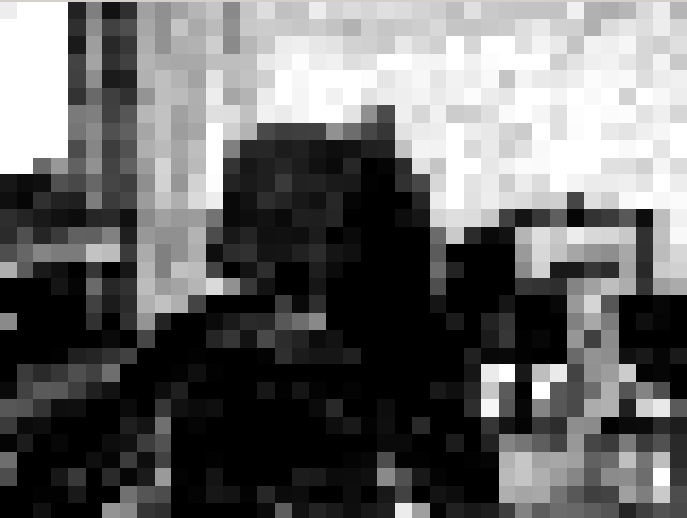
\includegraphics[scale=0.4]{PaulDefault120_91250kbps_psnr}
    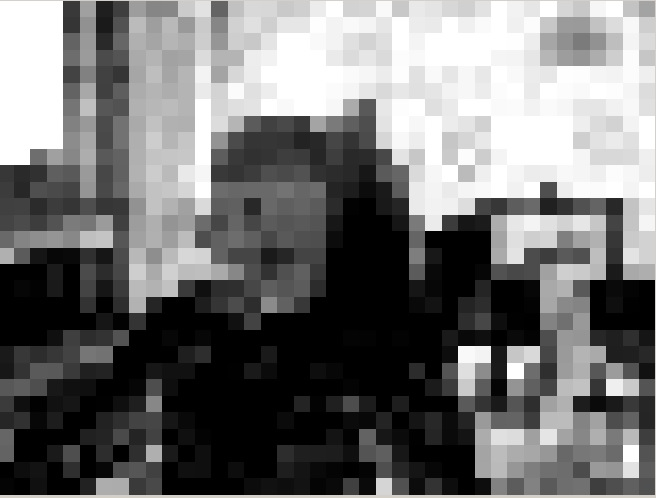
\includegraphics[scale=0.4]{BufferControl/paul120_250kbps_BufferControl_psnr}
    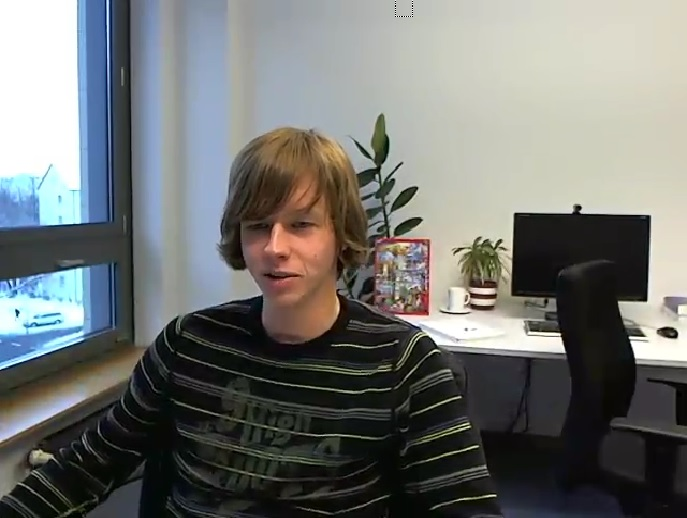
\includegraphics[scale=0.4]{PaulDefault120_91250kbps}
    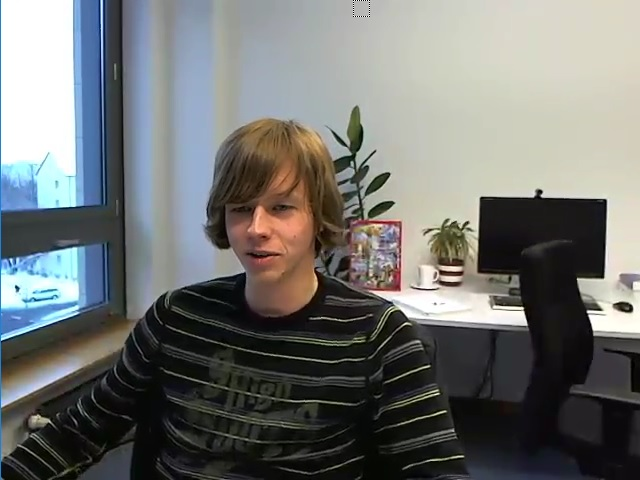
\includegraphics[scale=0.4]{BufferControl/paul120_250kbps_bufferControl}
    
\includegraphics[scale=0.37]{PaulDefault120_91250kbps_quant}
    
\includegraphics[scale=0.4]{BufferControl/paul120_250kbps_BufferControl_quant}    
    \caption{Comparing the images with modified reaction for ROI macroblcoks}
    \label{fig:Default_BufferControlCompare}
\end{figure}

The second approach of using the ROI information to enhance quality of ROI is by using different buffer controls inside the bitrate control module. The bitrate control module used in this study compensates for the overconsumption or underconsumption of bits in the past by adjusting the delta bits during bit allocation of the future frames. This corrected allocation happens at every macroblock level. For instance, if there is excessive consumption of bits in the past macro-blocks, the excess is subtracted from bit budget of certain number of future frames known as reaction factor. If the reaction factor is low, the excess or shortage of bits is shared by a large number of macro-blocks.

The reaction factor is used to allocate additional bits to ROI by using different reaction factors for macro-blocks belonging to the ROI. For instance, in case of underconsumption in the past, the excess bits available for future macroblocks is forced to be used aggressively for macroblocks belonging to ROI. On the other hand whenever there is overconsumption in the past, the bits are reduced more aggressively for macroblocks belonging to non-ROI. The advantage of this approach over QP offset approach is that the bit-allocation is still controlled within the rate control module and its decisions are not overridden by external offsets. This guarantees better buffer compliance. The results shown in Figure \ref{fig:Default_BufferControlCompare} compares the output with modified reaction factor based on region of interest and original video. It can be noticed that PSNR of the face regions is very close to that of the background. The data in Table \ref{AllPSNR1} shows that PSNR of ROI region is actually higher than the overall frame PSNR. The delay plots in \ref{fig:DelayDefault_BufferControltCompare} shows there is no significant changes in the delay or bitrate consumption.
%
%
%Bibiliography and reference
%
%
%
\clearpage
\begin{thebibliography}{9}
\bibitem{HighQualityROICodingForVideoConferencing} 
Manzur Murshed and James Brown. 
\textit{High Quality Region-of-Interest Coding for Video Conferencing based Remote General Practitioner Training}. 
The Fifth International Conference on eHealth, Telemedicine, and Social Medicine.

\bibitem{ComparingCodingEfficiency} 
J. Ohm. G. J. Sullivan, H. Schwarz, Thiow Keng Tan and T. Wiegand.
\textit{Comparison of the Coding Efficiency of Video Coding Standards—Including High Efficiency Video Coding (HEVC).}
 IEEE Transactions on Circuits and Systems for Video Technology ( Volume: 22, Issue: 12, Dec. 2012 )

\bibitem{JVTF086}
Siwei Ma, Wen Gao, Yan Lu and Hanqing Lu.
\textit{Proposed draft description of rate control on JVT standard. }
Joint Video Team (JVT) of ISO/IEC MPEG and ITU-T VCEG (ISO/IEC JTC1/SC29/WG11 and ITU-T SG16 Q.6) 6h Meeting: Awaji, 5-13, December, 2002.

\end{thebibliography}
\end{document}
